\chapter{Hardware Design}
\label{chp:DEM}
This chapter will discuss the detailed design of the device. Attention will be given to implementation of each component selected in the consent generation stage. The interface between the various sensors and the MCU will be discussed. The communication between the device and the PC and the software running on the MCU and on the PC will be laid out.

\section{Measure Heat Rate and Sp02}
Heart rate and \( SpO_2 \) will be measured with the same sensor: A pulse oximeter. 

As stated in the literature study, blood oxygen saturation can be measured through an arterial blood gas test or through pulse oximetry. Arterial blood gas test involves drawing a blood sample and doing in vitro tests on the sample. This method can be rejected, for it is in obvious violation of the system requirements. Pulse oximitry is therefore the preferred method for measuring \( SpO_2 \).

A pulse oximeter consists of two LEDs (emittors) and a photo detector. There are an few possible solutions that needs to be considered. Three set-ups are considered.

Firstly, the pulse oximeter in transmittance mode. The transmittance mode will require the emitters and detector to sit on opposite sides of a thin piece of tissue. A suitable location for this will be the ear lobule or the tragus. The cartilaginous pinna will not be ideal, for is contains less blood vessels.

Secondly, the inside of the ear canal is also considered. This set-up will consist of placing the emitters and detector on opposite walls of the ear canal. This set-up will combine reflective and transmittance modes, for light will be reflected and transmitted through the tissue around the ear canal from the ons side to the other. Figure X.

Lastly the pulse oxymeter in reflective mode. This mode allows the emitters and detector to be place next to each other. It need not be paced on a thin part of tissue. This means that the pulse oxymeter can be place against on side of the ear canal wall.



Figure~\ref{fig:PulseOxiConfiguration}

\begin{figure}
   \centering
   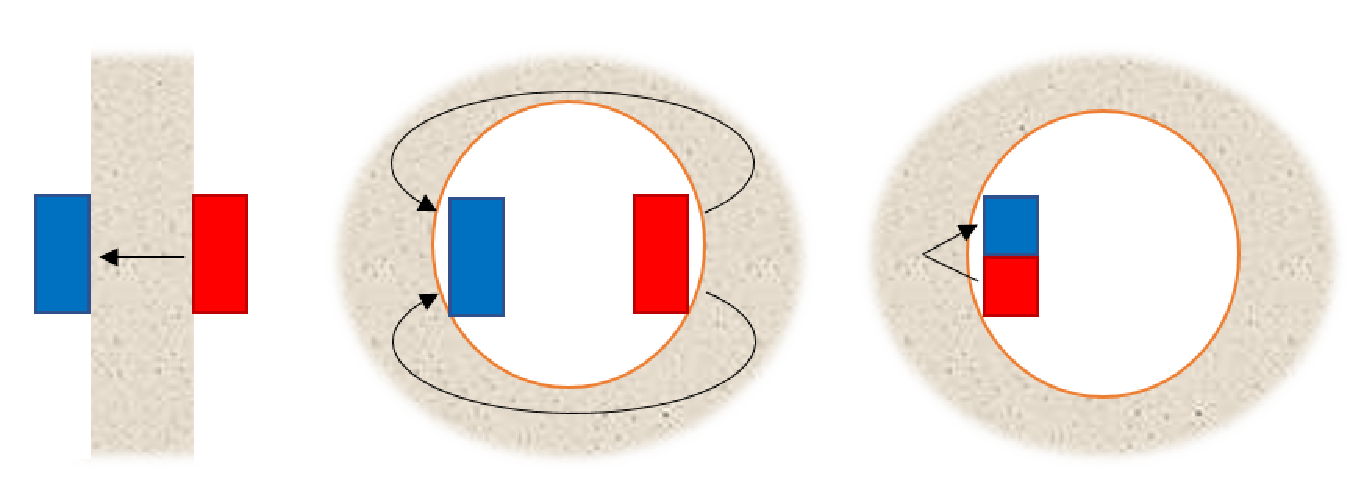
\includegraphics[scale=0.6]{figs/PulseOxiConfiguration}
   \caption{Drawing of the auricle (goo.gl/mmLnFx)}
   \label{fig:PulseOxiConfiguration}
\end{figure}

The pulse oxymeter in reflective mode was selecte.

Three hardware options: Custom components, NJL5501R and MAX30100

What methods and sensors was regarded. How was die MAX30100 selected at the end.



modulation ratio between red and infrared LED signals


\subsection{Thermometer Design}

Copy the Thermometer Subsystem word doc info in here, and the images.

Calibration information

Software design

The advantages of measuring the temperature of the tympanum has been discussed during the literature review. It has also been mentioned that measuring temperature through a thermistor (thermopile) in contact with the membrane can cause discomfort and harm to the wearer. Therefore an IR temperature sensor will be used to measure the tympanic temperature.

An understanding has been obtained about the general theory of IR thermo-sensing. This allows for the selection of a sensor to measure the tympanic temperature.

Various IR sensors are available. The main constraint for the sensor is the size. The sensor must be able to fit inside the ear canal of the wearer in order to have an unobstructed view of the tympanic membrane. This limits the options considerably. Two sensors were seriously considered: The TMP006 and the ...... The TMP006 is an non-contact IR sensor with a digital interface. (More general sensor description information from the data sheet here)

The (other sensor info)
How the TMP006 choice was made at the end















%%SOFTEWARE DESIGN - DIFFERENT SECTION
\subsection{MAX30100 flow of data}
This section will explain how data flows from the MAX30100 to the user interface and how specific vital sign information is extracted.

adaptative treshold

\subsubsection{AC and DC Extraction}
As mentioned in the detailed design section, the MAX30100 converts reflected light intensity to voltage level which in turn is converted to an 16-bit? integer through an on chip ADC. This digital value is a representation of the amount of light reflected by the tissue of the ear canal. This value contains a DC and AC component. The AC component contains the pulse information. The DC components is used in calculating Sp02? and to adjust the current through the red LED on the MAX30100 (see dynamic current adjustment subsubsection) To separate the AC and DC components a IIR filter is implemented on the MCU.

Give the formula and explain what the variables are (see design word doc)

Choosing alpha close to one will create a filter with a narrow stop band close to the DC frequency. Through some trail and error an alpha value of ? was chosen. Criteria for this choice was signal form and steady DC rejection, less drift?? (Insert some graphs plotted of filtered signals with different alpha values, maby also a frequancy response graph of the filter)

\subsubsection{Dynamic LED Current Adjustment}
The MAX30100 allows for the individual adjustment of red and IR LED currents (get better description from data sheet). This ability can be used to improve the accuracy of the Sp02 calculation. 


\subsubsection{Beat Detection}
The absorption spectra of oxygenated blood is highest for IR light. Therefore IR light is used to obtain the PPG.

See Pulse-Peak Detection of Wearable Sensing of In-Ear Pressure for Heart Rate Monitoring with a Piezoelectric Sensor saved article

\subsubsection{Sp02 Calculation}
After the AC component has been extracted from the signal is is possible to calculate the $SpO_2$. An AC root mean square is calculated of the red and IR signals over a period of 5 heart beats (why). The ratio between the red and IR RMS valus are then calculated and the \%$SpO_2$ is calculated with the standard formula from literature. The following formula describes the calculation: $$\%SpO_2 = 110-25\left(\frac{Red ACrms}{IR ACrms}\right)$$

\subsubsection{Measure Heat Rate and Sp02}

\subsubsection{Measure Breathing Rate}




\subsubsection{Measure EEG}